\chapter{Image Pages}

\lipsum[1-5]

\clearpage

{
\parindent0pt
\pagestyle{empty}

\fboxsep0pt
\fboxrule0pt

\vspace*{-1cm}
\begin{minipage}{1.05\textwidth}
\hskip-0.9cm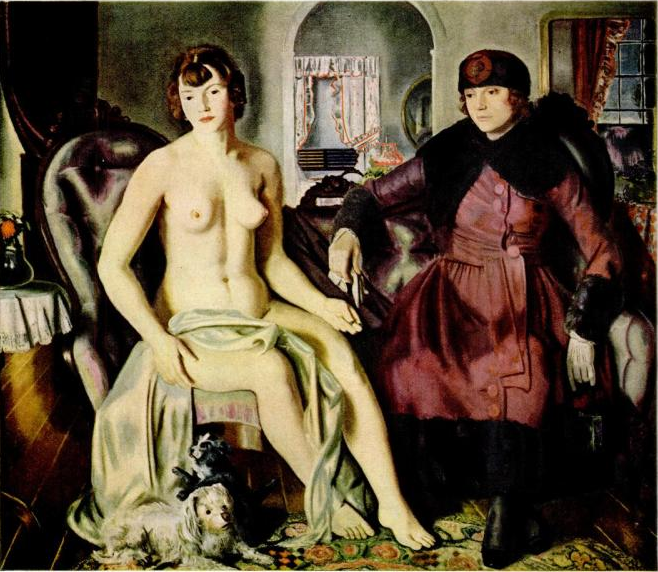
\includegraphics[width=1.03\textwidth]{twowomen-03}\\[-27.5pt]
\setlength{\linewidth}{0.95\textwidth}
\setlength{\columnsep}{10pt}
\begin{multicols}{2}
\noindent \footnotesize\textbf{TWO WOMEN,} portrays a professional model dressed and undressed. The range and richness of colors is unusual among Bellows' pictures. Bellows always had a horror of studio pictures and ``pretty nudes.'' He rarely worked from professional models and never painted a still life. This painting was published in Life Magazine.
\end{multicols}
\vspace{-0.25cm}
\rule{1.5cm}{0pt}\fbox{
\begin{minipage}[t]{0.87\textwidth}
\begin{minipage}[t]{0.41\textwidth}
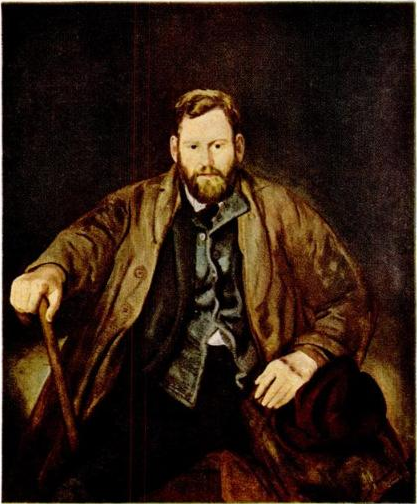
\includegraphics[width=1.03\textwidth]{threewomen01}\par\vspace*{-8pt}%
\captionof*{figure}{\noindent\footnotesize\textbf{WALDO PEIRCE}, a famous painting in his own right,
turned model for Bellows, posed for this impressive portrait in New York studio in 1920.}
\end{minipage}\hspace{0.5cm}
\begin{minipage}[t]{0.4\textwidth}
   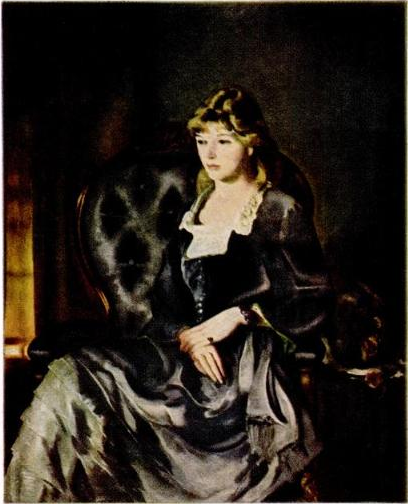
\includegraphics[width=1\textwidth]{threewomen02}\vspace*{-8pt}
    \captionof*{figure}{\noindent\footnotesize\textbf{Mrs Katherine Rosen,}
the daughter of Charles Rosen, he was an artist and neighbor of bellows, posed for this meditative study in 1921.}
\end{minipage}
\end{minipage}
}

\vfill

\captionof{figure}{Balancing three images on a page. Should the larger image be at the top or at the bottom?}
\end{minipage}
}

